\section{Multi-Leader репликация. Last Write Wins.}
    Один из способов решения конфликта --- оставлять на каждой реплике только последнюю (в некотором смысле) запись. Нельзя на каждой реплике сохранять последнюю пришедшую запись, потому что тогда, они даже \textit{eventually} не придут к согласованности.
    \begin{itemize}
        \item Физические часы --- каждая запись будет иметь метку времени --- физическое время той реплики, которая приняла эту запись, но из-за плохо синхронизированных часов может отбросить последнюю запись, хотя последнюю надо оставлять.
        \item Логические часы --- векторные часы, основанные на отношении ``произошло до``, но среди параллельных записей нет той, которая произошла до, и брать любую из них тоже нельзя.
    \end{itemize}
      \begin{definition}
        Метод \textit{Last Write Wins} не работает при выборе любой из параллельных записей.\\
          $c$ happens-before $b$, $a \parallel b$, $a \parallel c$. \\
          Приоритет по убыванию: $c$, $b$, $a$. \\
          \begin{itemize}
          \item При конфликте берем покомпонентый максимум векторных версий:
            \begin{itemize}
              \item $a + c = c, a + c \parallel b$
              \item $(a + c) + b = a + c = c$
              \item $a + b = a, c \rightarrow (a + b)$
              \item $(a + b) + c = a + b = a$
            \end{itemize}
          \item При конфликте берем версию победителя:
          \begin{itemize}
            \item $a + c = c, (a + c) \rightarrow b$
            \item $(a + c) + b = b$
            \item $a + b = a, (a + b) \parallel c$
            \item $(a + b) + c = c$
          \end{itemize}
         \item Поэтому держать только актуальное значение на реплике, и заменять при необходимости на нужное не получится.
        \end{itemize}
      \end{definition}
        \begin{algorithm}(Решение конфликтов)
          \begin{itemize}
            \item Для каждого ключа на каждой реплики храним $N$ значений --- последнее полученное с каждой из $N$ реплик значение по соответствующему ключу.
            \item Когда хотим получить актуальное значение, строим множество $W$, в котором оставим только параллельные операции, а те которое связаны хоть с кем-то отношением ``произошло до`` выкинем, среди этого множествва оставим одно значение произвольным образом, например по timestamp'у.
          \end{itemize}
        \end{algorithm}
    \begin{remark}
      Серьезная проблема --- понимать, когда и какую из старых операций можно забыть.
    \end{remark}
    \begin{example}
      \begin{figure}[h]
          \centering
          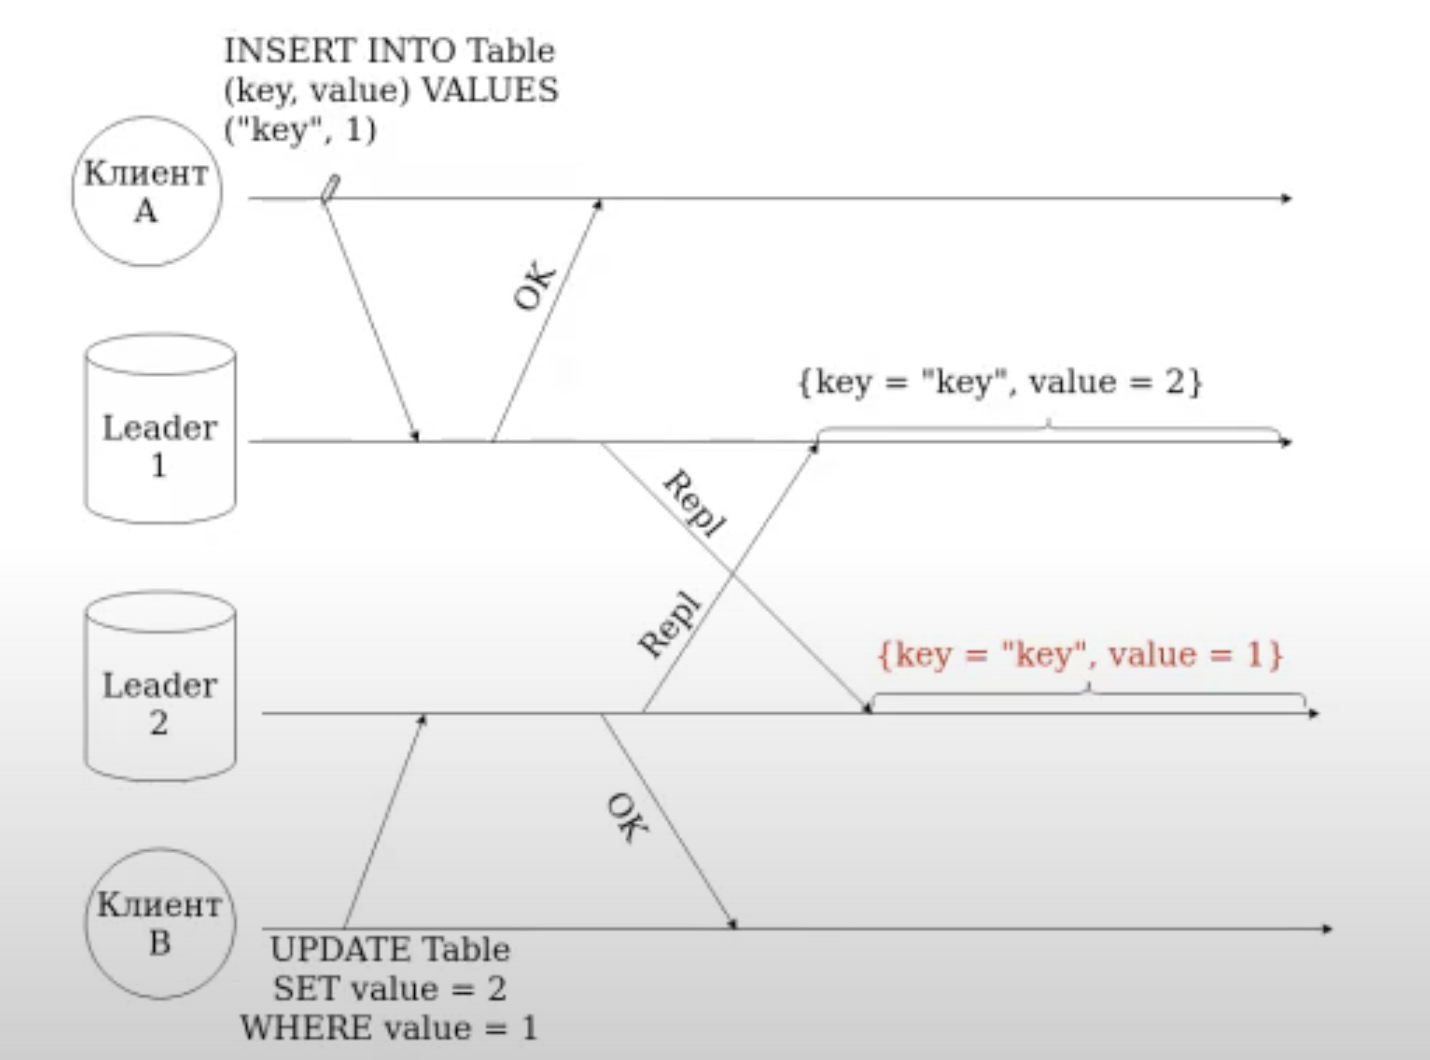
\includegraphics[scale = 0.5]{../assets/14.png}
          \caption{Пример для РСУБД}
      \end{figure}
      Даже если в операции не упоминается явно ключ --- не значит, что можно забыть.\\
    \end{example}
    \begin{example}
      Инкрементор:\\
        \begin{itemize}
          \item Состояние --- единственное число.
          \item Система выполняет запросы вида ``увеличить число на k``.
          \item Если не храним предка пришедшей записи, то мы не можем сказать, на сколько увеличил третий узел.
          \item \begin{figure}[h]
                        \centering
                        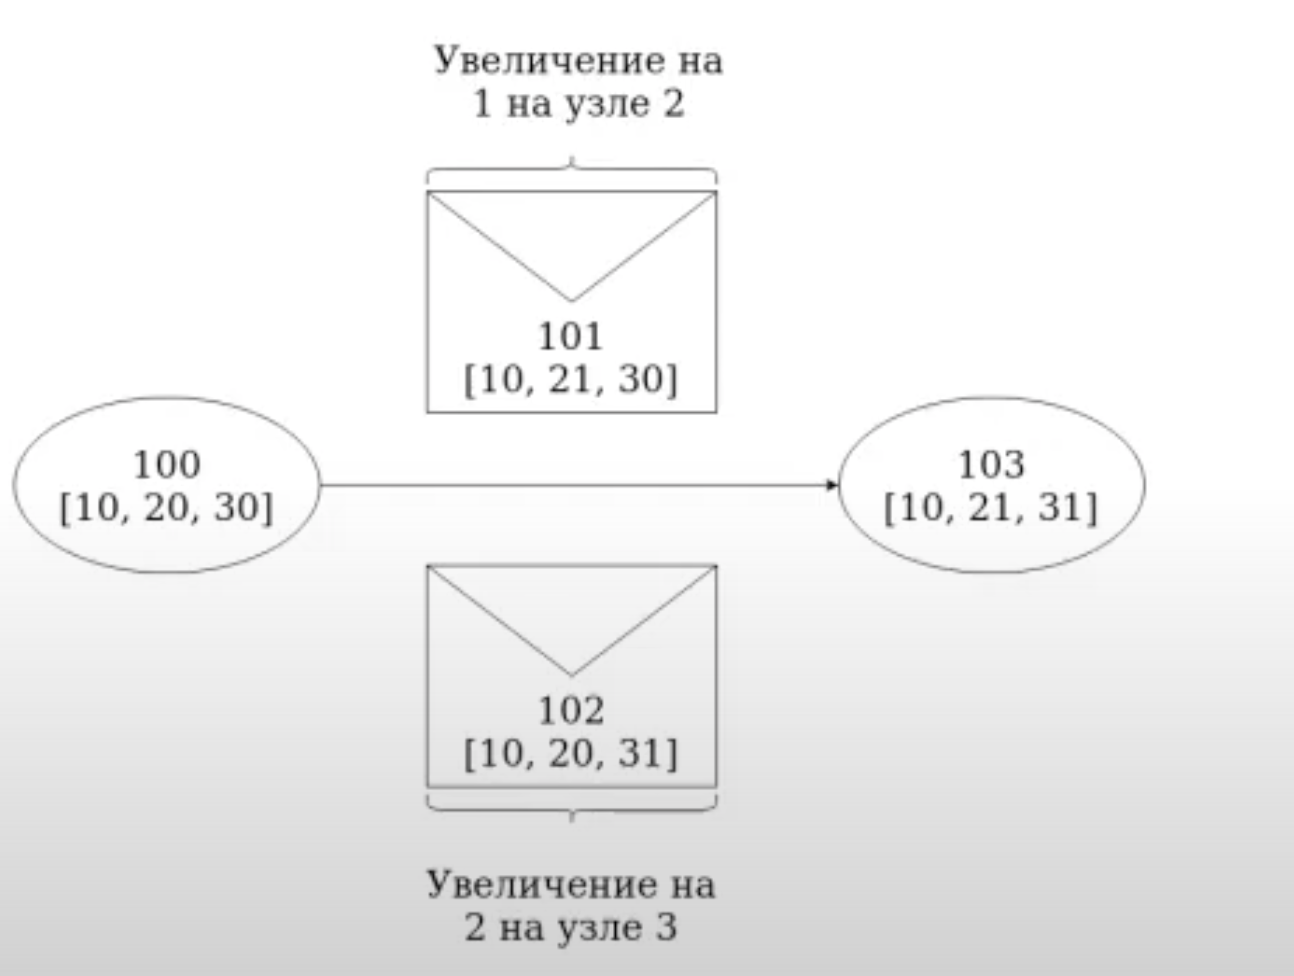
\includegraphics[scale = 0.5]{../assets/15.png}
                        \caption{Параллельная запись}
                \end{figure}
          \item \begin{figure}[h]
                        \centering
                        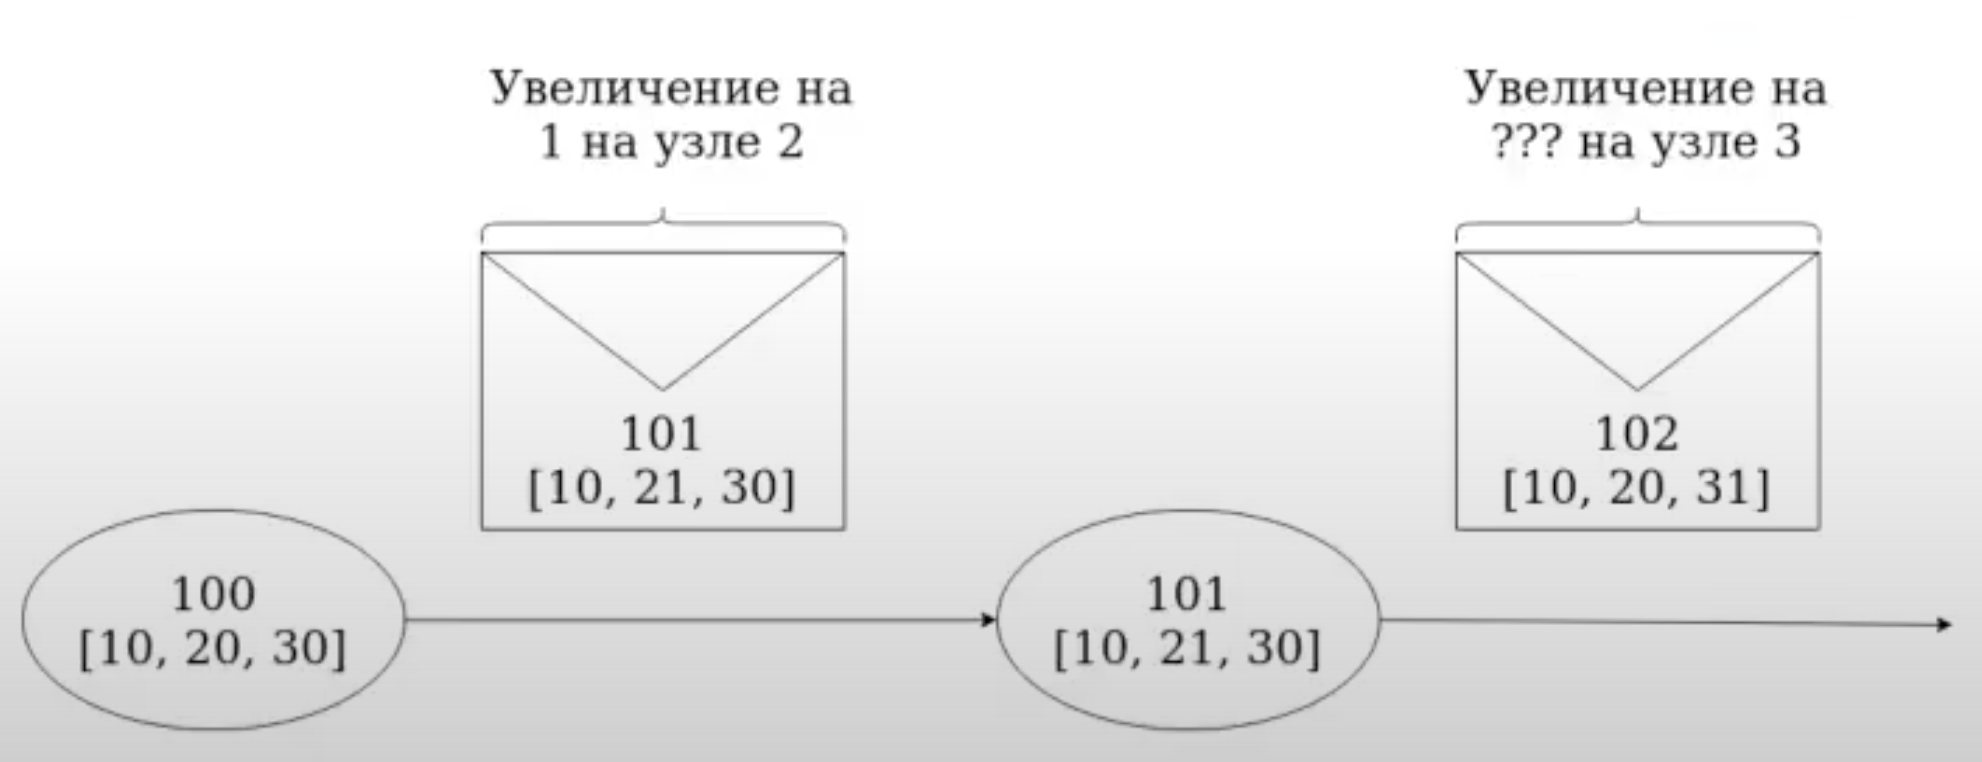
\includegraphics[scale = 0.5]{../assets/16.png}
                        \caption{Последовательная запись}
                \end{figure}
          \item Храним старое состояние, пока имеется возможность получить его непосредственного потомка.
          \item Выкидываем старое, когда по каждой компоненте вектора $V$ получили ``следующее`` состояние.
      \end{itemize}
    \end{example}
